\section{Результаты}
\subsection{Выборочные коэффициенты корреляции}
\begin{table}[H]
	\centering
	\begin{tabular}{|c|c|c|c|}
\hline
$\rho = 0~(\ref{ro})$ & $r ~(\ref{r})$ & $r_Q ~(\ref{rQ})$ & $r_S ~(\ref{rS})$\\
\hline
$E(z)$ & -0.0 & -0.001 & -0.006\\
\hline
$E(z^2)$ & 0.054 & 0.055 & 0.055\\
\hline
$D(z)$ & 0.233 & 0.234 & 0.235\\
\hline
$\rho = 0.5~(\ref{ro})$ & $r ~(\ref{r})$ & $r_Q ~(\ref{rQ})$ & $r_S ~(\ref{rS})$\\
\hline
$E(z)$ & 0.479 & 0.45 & 0.314\\
\hline
$E(z^2)$ & 0.263 & 0.241 & 0.149\\
\hline
$D(z)$ & 0.184 & 0.197 & 0.225\\
\hline
$\rho = 0.9~(\ref{ro})$ & $r ~(\ref{r})$ & $r_Q ~(\ref{rQ})$ & $r_S ~(\ref{rS})$\\
\hline
$E(z)$ & 0.896 & 0.868 & 0.7\\
\hline
$E(z^2)$ & 0.806 & 0.759 & 0.518\\
\hline
$D(z)$ & 0.051 & 0.07 & 0.169\\
\hline
\end{tabular}
	\caption{Двумерное нормальное распределение, n = 20}
	\label{tab:n20}
\end{table}
\begin{table}[H]
	\centering
	\begin{tabular}{|c|c|c|c|}
\hline
$\rho = 0~(\ref{ro})$ & $r ~(\ref{r})$ & $r_Q ~(\ref{rQ})$ & $r_S ~(\ref{rS})$\\
\hline
$E(z)$ & -0.009 & -0.007 & -0.004\\
\hline
$E(z^2)$ & 0.017 & 0.017 & 0.018\\
\hline
$D(z)$ & 0.131 & 0.132 & 0.133\\
\hline
$\rho = 0.5~(\ref{ro})$ & $r ~(\ref{r})$ & $r_Q ~(\ref{rQ})$ & $r_S ~(\ref{rS})$\\
\hline
$E(z)$ & 0.498 & 0.477 & 0.33\\
\hline
$E(z^2)$ & 0.258 & 0.239 & 0.123\\
\hline
$D(z)$ & 0.101 & 0.105 & 0.119\\
\hline
$\rho = 0.9~(\ref{ro})$ & $r ~(\ref{r})$ & $r_Q ~(\ref{rQ})$ & $r_S ~(\ref{rS})$\\
\hline
$E(z)$ & 0.898 & 0.883 & 0.705\\
\hline
$E(z^2)$ & 0.808 & 0.78 & 0.506\\
\hline
$D(z)$ & 0.025 & 0.033 & 0.093\\
\hline
\end{tabular}
	\caption{Двумерное нормальное распределение, n = 60}
	\label{tab:n60}
\end{table}
\begin{table}[H]
	\centering
	\begin{tabular}{|c|c|c|c|}
\hline
$\rho = 0~(\ref{ro})$ & $r ~(\ref{r})$ & $r_Q ~(\ref{rQ})$ & $r_S ~(\ref{rS})$\\
\hline
$E(z)$ & -0.001 & 0.001 & 0.001\\
\hline
$E(z^2)$ & 0.011 & 0.011 & 0.01\\
\hline
$D(z)$ & 0.106 & 0.106 & 0.101\\
\hline
$\rho = 0.5~(\ref{ro})$ & $r ~(\ref{r})$ & $r_Q ~(\ref{rQ})$ & $r_S ~(\ref{rS})$\\
\hline
$E(z)$ & 0.5 & 0.48 & 0.328\\
\hline
$E(z^2)$ & 0.256 & 0.236 & 0.117\\
\hline
$D(z)$ & 0.076 & 0.079 & 0.094\\
\hline
$\rho = 0.9~(\ref{ro})$ & $r ~(\ref{r})$ & $r_Q ~(\ref{rQ})$ & $r_S ~(\ref{rS})$\\
\hline
$E(z)$ & 0.898 & 0.885 & 0.709\\
\hline
$E(z^2)$ & 0.807 & 0.784 & 0.507\\
\hline
$D(z)$ & 0.019 & 0.024 & 0.072\\
\hline
\end{tabular}
	\caption{Двумерное нормальное распределение, n = 100}
	\label{tab:n100}
\end{table}
\begin{table}[H]
	\centering
	\begin{tabular}{|c|c|c|c|}
\hline
$n = 20$ & $r ~(\ref{r})$ & $r_Q ~(\ref{rQ})$ & $r_S ~(\ref{rS})$\\
\hline
$E(z)$ & 0.802 & 0.768 & 0.587\\
\hline
$E(z^2)$ & 0.651 & 0.601 & 0.378\\
\hline
$D(z)$ & 0.092 & 0.108 & 0.182\\
\hline
$n = 60$ & $r ~(\ref{r})$ & $r_Q ~(\ref{rQ})$ & $r_S ~(\ref{rS})$\\
\hline
$E(z)$ & 0.809 & 0.788 & 0.593\\
\hline
$E(z^2)$ & 0.656 & 0.623 & 0.362\\
\hline
$D(z)$ & 0.045 & 0.052 & 0.102\\
\hline
$n = 100$ & $r ~(\ref{r})$ & $r_Q ~(\ref{rQ})$ & $r_S ~(\ref{rS})$\\
\hline
$E(z)$ & 0.809 & 0.791 & 0.6\\
\hline
$E(z^2)$ & 0.655 & 0.627 & 0.367\\
\hline
$D(z)$ & 0.035 & 0.042 & 0.082\\
\hline
\end{tabular}
	\caption{Смесь нормальных распределений}
	\label{tab:mix}
\end{table}

\subsection{Эллипсы рассеивания}
\begin{flushleft}
	Для уравнения эллипса выбиралась константа $const = 9$.
\end{flushleft}
\begin{figure}[H]
	\center{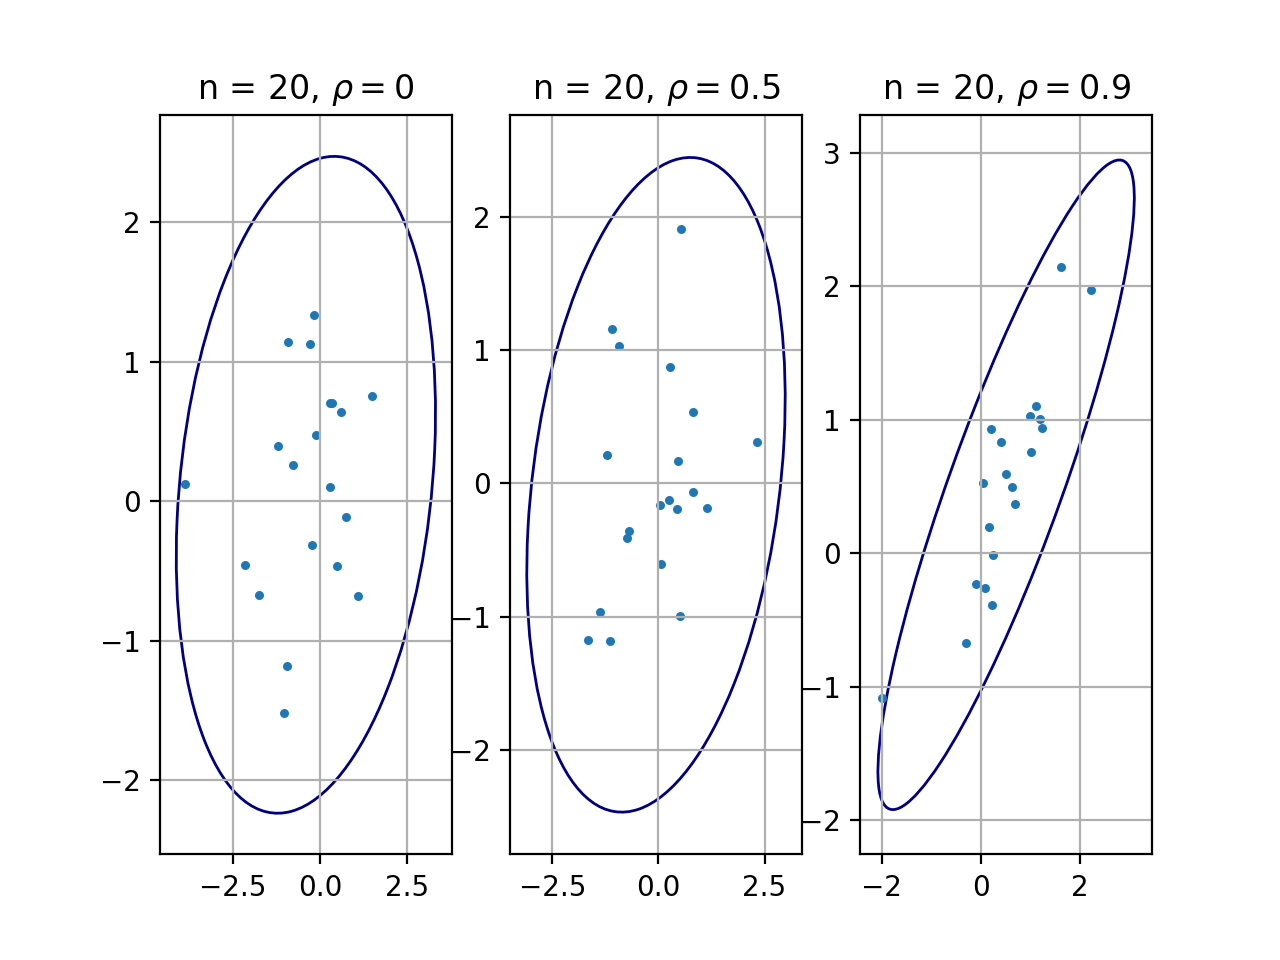
\includegraphics[width=1\linewidth]{task1\_data/20}}
	\caption{Двумерное нормальное распределение, $n$ = 20}
	\label{fig:n20}
\end{figure}
\begin{figure}[H]
	\center{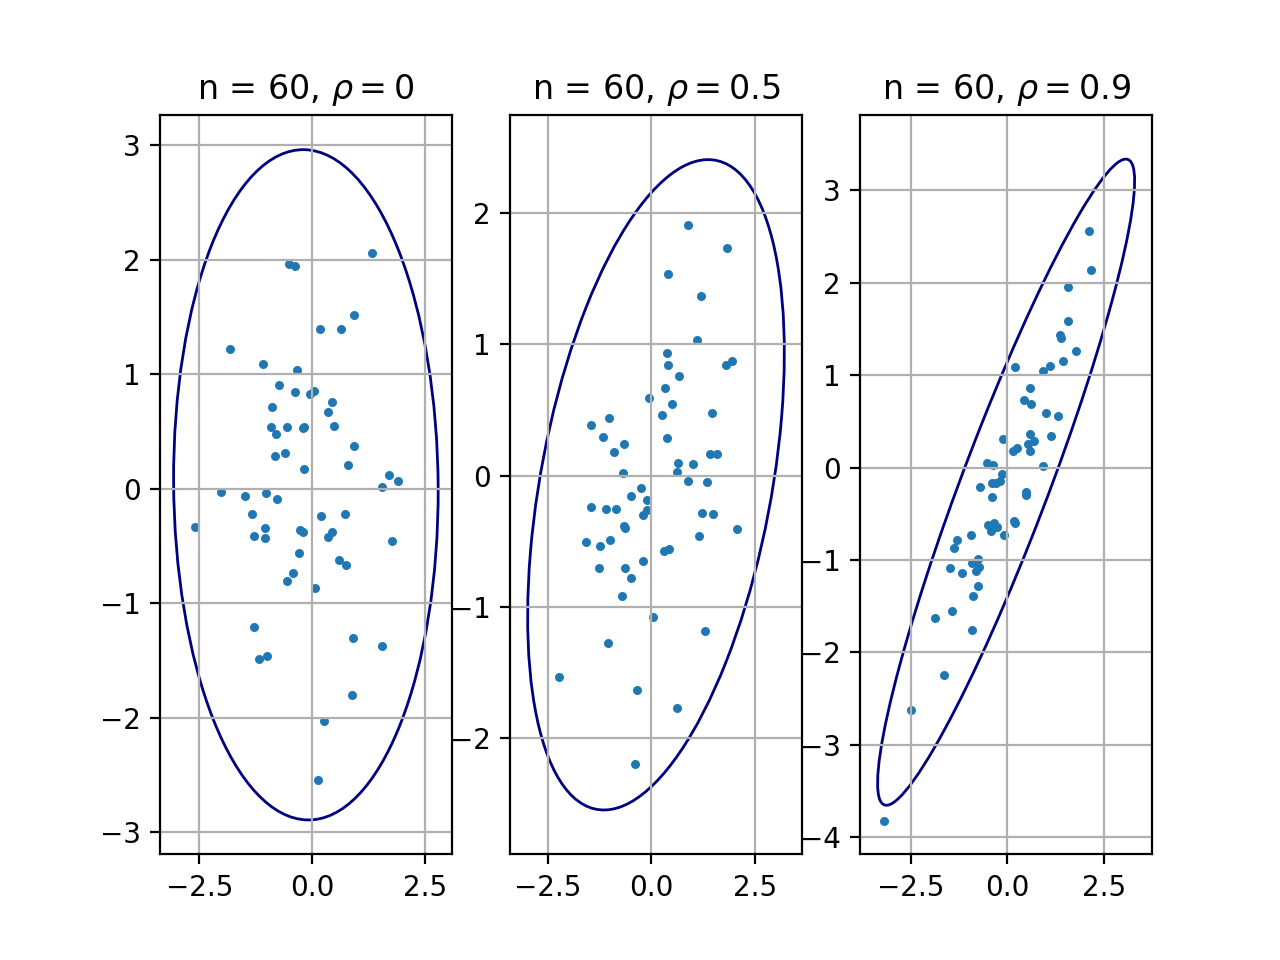
\includegraphics[width=1\linewidth]{task1\_data/60}}
	\caption{Двумерное нормальное распределение, $n$ = 60}
	\label{fig:n60}
\end{figure}
\begin{figure}[H]
	\center{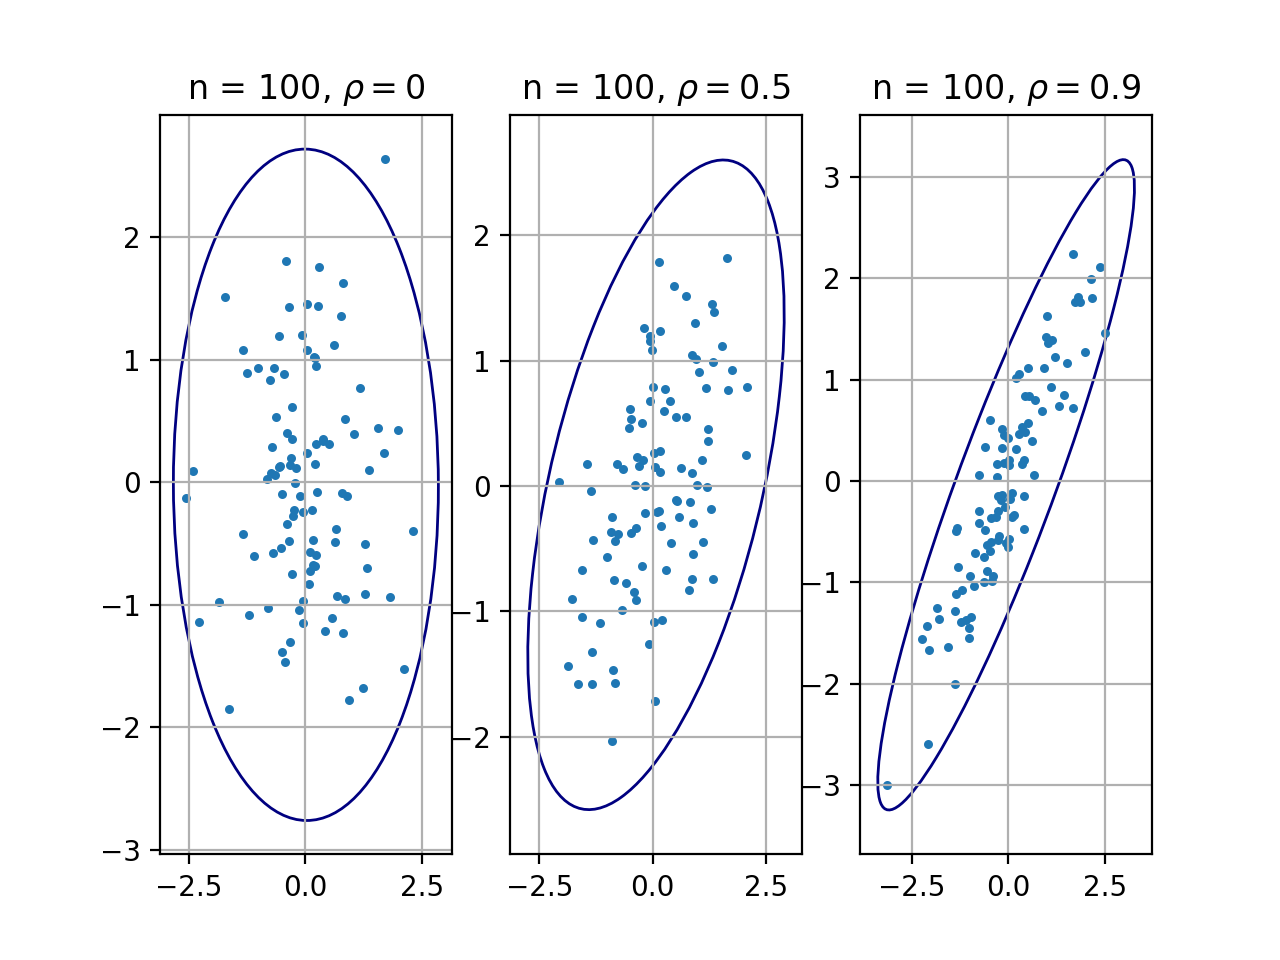
\includegraphics[width=1\linewidth]{task1\_data/100}}
	\caption{Двумерное нормальное распределение, $n$ = 100}
	\label{fig:n100}
\end{figure}
\begin{figure}[H]
	\center{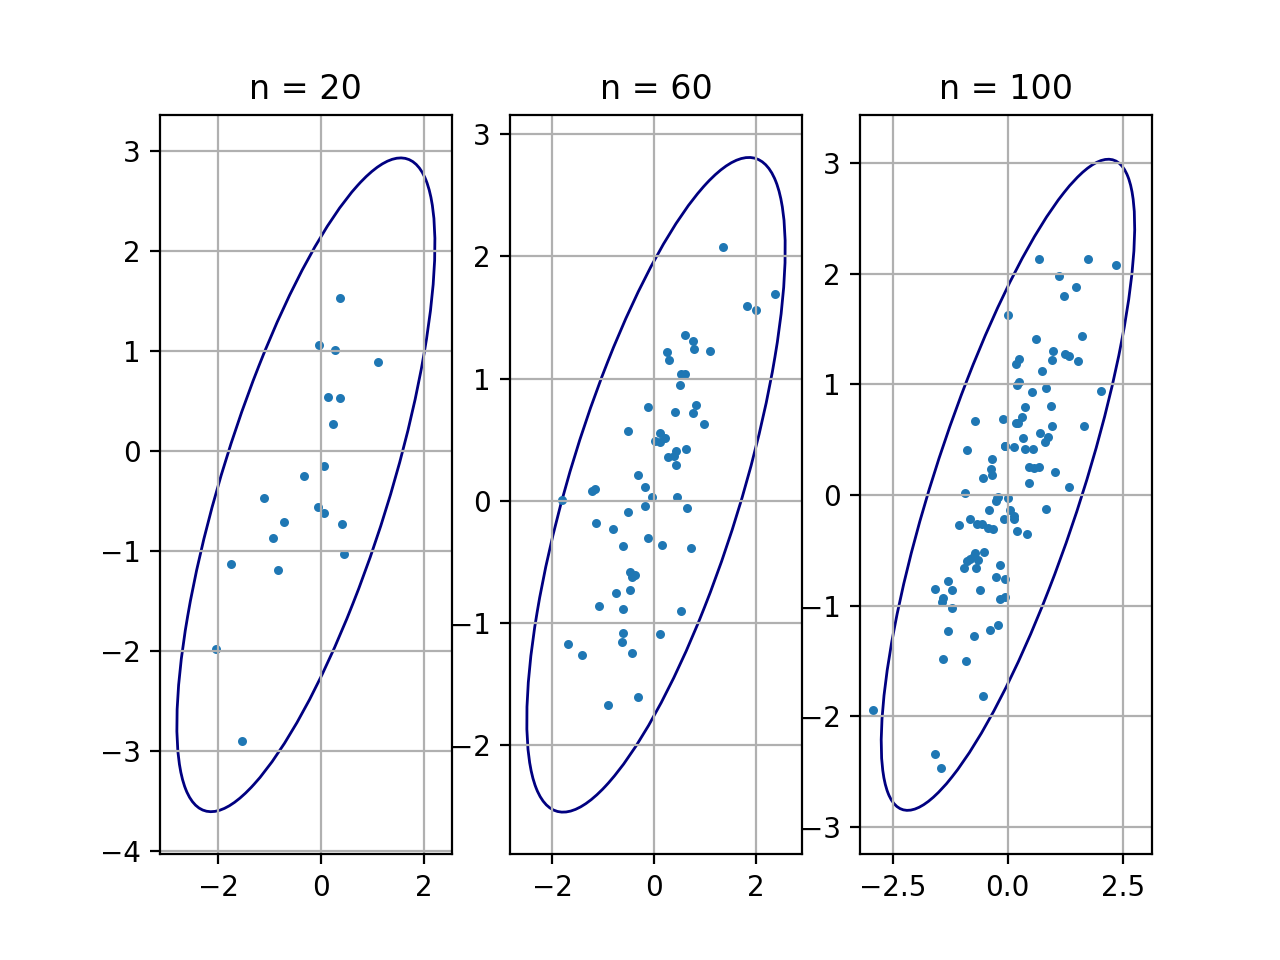
\includegraphics[width=1\linewidth]{task1\_data/mix}}
	\caption{Смесь нормальных распределений}
	\label{fig:mix}
\end{figure}

\subsection{Оценки коэффициентов линейной регрессии}
\subsubsection{Выборка без возмущений}
\begin{flushleft}
	\begin{enumerate}
\item МНК, без возмущений:
$\hat{a}\approx 1.9408681061135704$, $\hat{b}\approx 2.011129422595325$
\item МНМ, без возмущений:
$\hat{a}\approx 1.6871749684086914$, $\hat{b}\approx 2.188840631442489$
\end{enumerate}

\end{flushleft}
\begin{figure}[H]
	\center{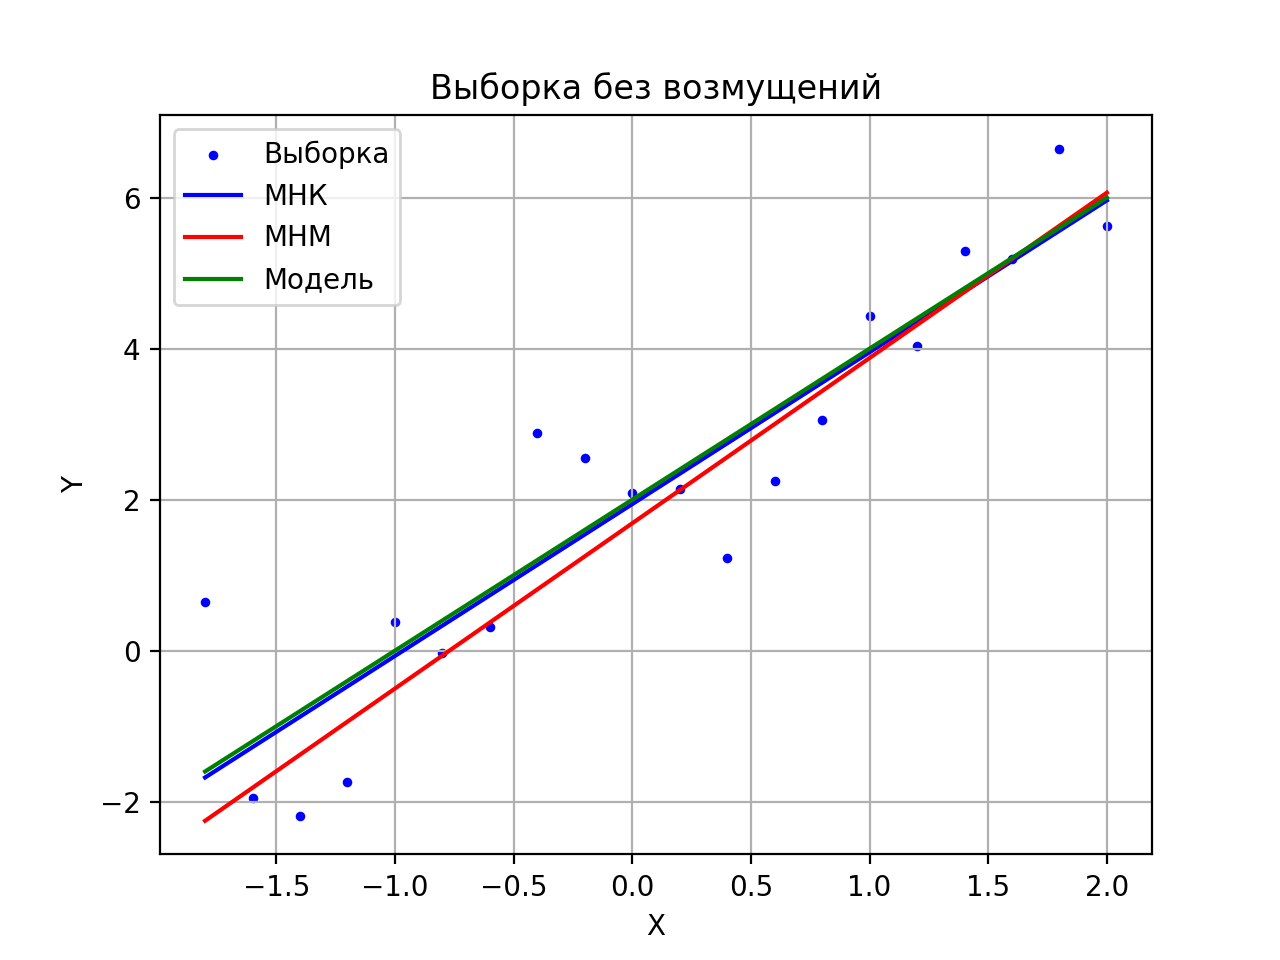
\includegraphics[width=1\linewidth]{task2\_data/no_noise}}
	\caption{Выборка без возмущений}
	\label{fig:no_noise}
\end{figure}
\subsubsection{Выборка с возмущениями}
\begin{flushleft}
	\begin{enumerate}
\item МНК, с возмущенями:
$\hat{a}\approx 2.0837252489707123$, $\hat{b}\approx 0.5825579940238962$
\item МНМ, с возмущенями:
$\hat{a}\approx 1.669124968837086$, $\hat{b}\approx 2.200173829809759$
\end{enumerate}

\end{flushleft}
\begin{figure}[H]
	\center{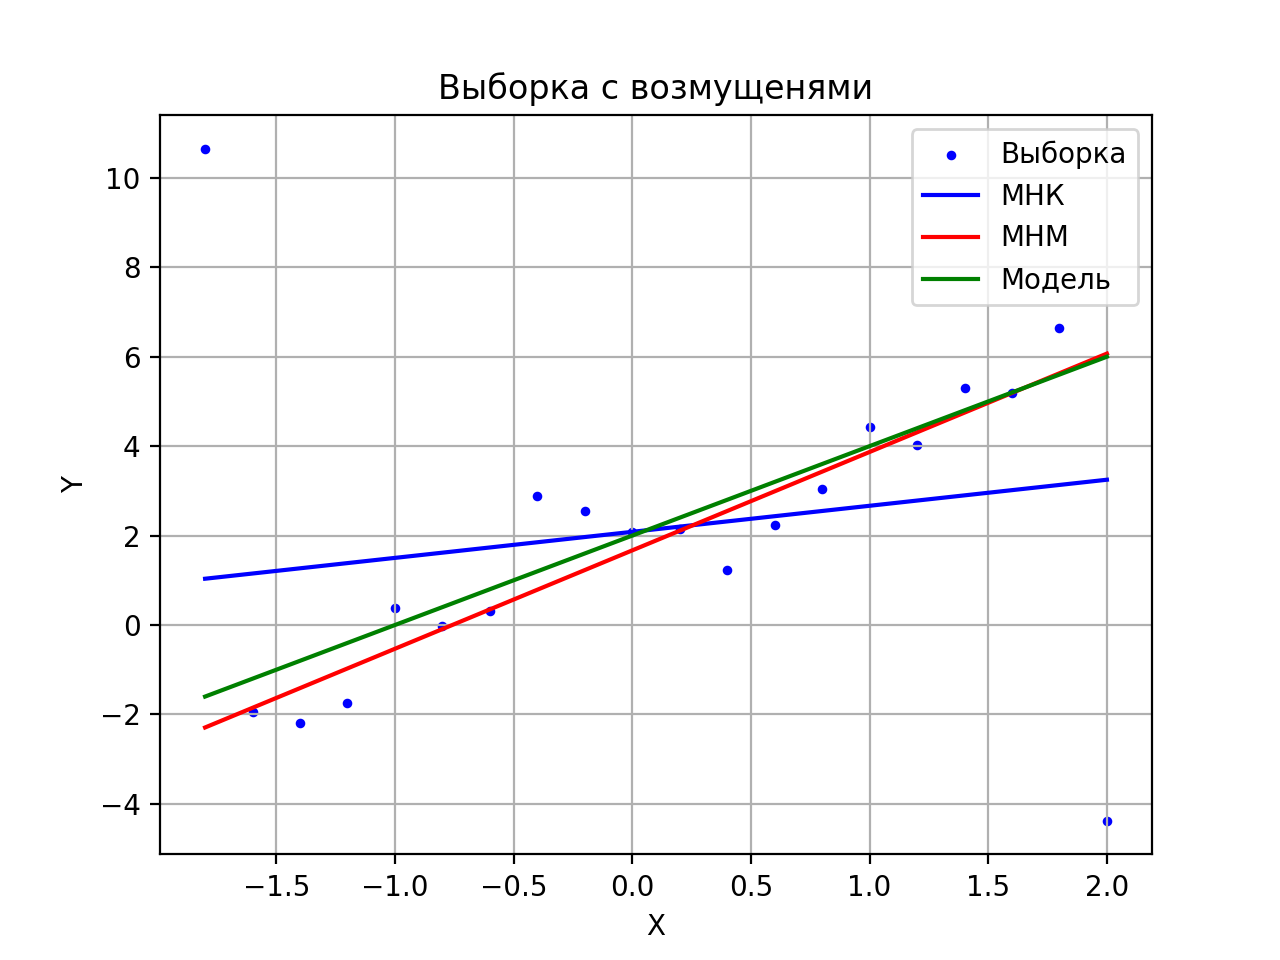
\includegraphics[width=1\linewidth]{task2\_data/noise}}
	\caption{Выборка с возмущениями}
	\label{fig:noise}
\end{figure}

\subsection{Проверка гипотезы о законе распределения генеральной совокупности. Метод хи-квадрат}
\begin{flushleft}
	Метод максимального правдоподобия: 
	$\hat{\mu} \approx -0.08, \hat{\sigma} \approx 0.96$\\
	\begin{table}[H]
		\centering
		\begin{tabular}{|c|c|c|c|c|c|c|}
\hline
\hline i & Границы $\Delta_i$ & $n_i$ & $p_i$ & $np_i$ & $n_i - np_i$ & $\frac{(n_i - np_i)^2}{np_i}$\\
\hline
1 & $-\inf$, -3.03 & 0.00 & 0.0013 & 0.13 & -0.13 & 0.13\\
\hline
2 & -3.03, -1.83 & 6.00 & 0.0339 & 3.39 & 2.61 & 2.00\\
\hline
3 & -1.83, -0.63 & 23.00 & 0.2380 & 23.80 & -0.80 & 0.03\\
\hline
4 & -0.63, 0.57 & 45.00 & 0.4535 & 45.35 & -0.35 & 0.00\\
\hline
5 & 0.57, 1.77 & 24.00 & 0.2380 & 23.80 & 0.20 & 0.00\\
\hline
6 & 1.77, 2.97 & 2.00 & 0.0339 & 3.39 & -1.39 & 0.57\\
\hline
7 & 2.97, $+\inf$ & 0.00 & 0.0013 & 0.13 & -0.13 & 0.13\\
\hline
$\sum$ & $-$ & 100.00 & 1.0000 & 100.00 & 0.00 & 2.86\\
\hline
\end{tabular}
		\caption{ Вычисление $\chi^{2}_{B}$ при проверке гипотезы $H_{0}$ о нормальном законе распределения $N(x,\hat{\mu}, \hat{\sigma})$}
		\label{tab:normal_chi_2}
	\end{table}
	Видим, что $\chi^{2}_{B} < \chi^{2}_{0.95} \approx 14.1$, следовательно, гипотезу полагаем верной.\\
	\begin{table}[H]
		\centering
		\begin{tabular}{|c|c|c|c|c|c|c|}
\hline
\hline i & Границы $\Delta_i$ & $n_i$ & $p_i$ & $np_i$ & $n_i - np_i$ & $\frac{(n_i - np_i)^2}{np_i}$\\
\hline
1 & $-\inf$, -3.34 & 0.00 & 0.0006 & 0.01 & -0.01 & 0.01\\
\hline
2 & -3.34, -2.14 & 1.00 & 0.0248 & 0.50 & 0.50 & 0.51\\
\hline
3 & -2.14, -0.94 & 4.00 & 0.2321 & 4.64 & -0.64 & 0.09\\
\hline
4 & -0.94, 0.26 & 9.00 & 0.4851 & 9.70 & -0.70 & 0.05\\
\hline
5 & 0.26, 1.46 & 5.00 & 0.2321 & 4.64 & 0.36 & 0.03\\
\hline
6 & 1.46, 2.66 & 1.00 & 0.0248 & 0.50 & 0.50 & 0.51\\
\hline
7 & 2.66, $+\inf$ & 0.00 & 0.0006 & 0.01 & -0.01 & 0.01\\
\hline
$\sum$ & $-$ & 20.00 & 1.0000 & 20.00 & 0.00 & 1.21\\
\hline
\end{tabular}
		\caption{Вычисление $\chi^{2}_{B}$ при проверке гипотезы $H_{0}$ о законе распределения $L(x,\hat{\mu}, \hat{\sigma})$, $n=20$}
		\label{tab:laplace_chi_2}
	\end{table}
	Видим, что $\chi^{2}_{B} < \chi^{2}_{0.95} \approx 14.1$, следовательно, гипотеза принимается и в этот раз.
\end{flushleft}

\subsection{Доверительные интервалы для параметров нормального распределения}
\begin{table}[H]
	\centering
	\begin{tabular}{| c | c | c |}
		\hline
		n = 20   &  $m$  & $\sigma$\\ \hline
		&  -0.38 < $m$ < 0.75 & 0.88 < $\sigma$ < 1.69 \\ \hline
		&   &   \\ \hline
		n = 100   &  $m$  & $\sigma$\\ \hline
		& -0.02 < $m$ < 0.40 & 0.95 < $\sigma$ < 1.25 \\
		\hline
	\end{tabular}
	\caption{Доверительные интервалы для параметров нормального распределения}
	\label{tab:interv_simple}
\end{table}

\subsection{Доверительные интервалы для параметров произвольного распределения. Асимптотический подход}
\begin{table}[H]
	\centering
	\begin{tabular}{| c | c | c |}
		\hline
		n = 20   &  $m$  & $\sigma$\\ \hline
		&  -0.29 < $m$ < 0.70 & 0.83 < $\sigma$ < 2.73 \\ \hline
		&   &   \\ \hline
		n = 100   &  $m$  & $\sigma$\\ \hline
		& -0.02 < $m$ < 0.40 & 0.90 < $\sigma$ < 1.42 \\
		\hline
	\end{tabular}
	\caption{Доверительные интервалы для параметров произвольного распределения. Асимптотический подход}
	\label{tab:interv_asimpt}
\end{table}

\subsection{Сравнение результатов 4.5 и 4.6. Графическое представление}
\begin{figure}[H]
	\center{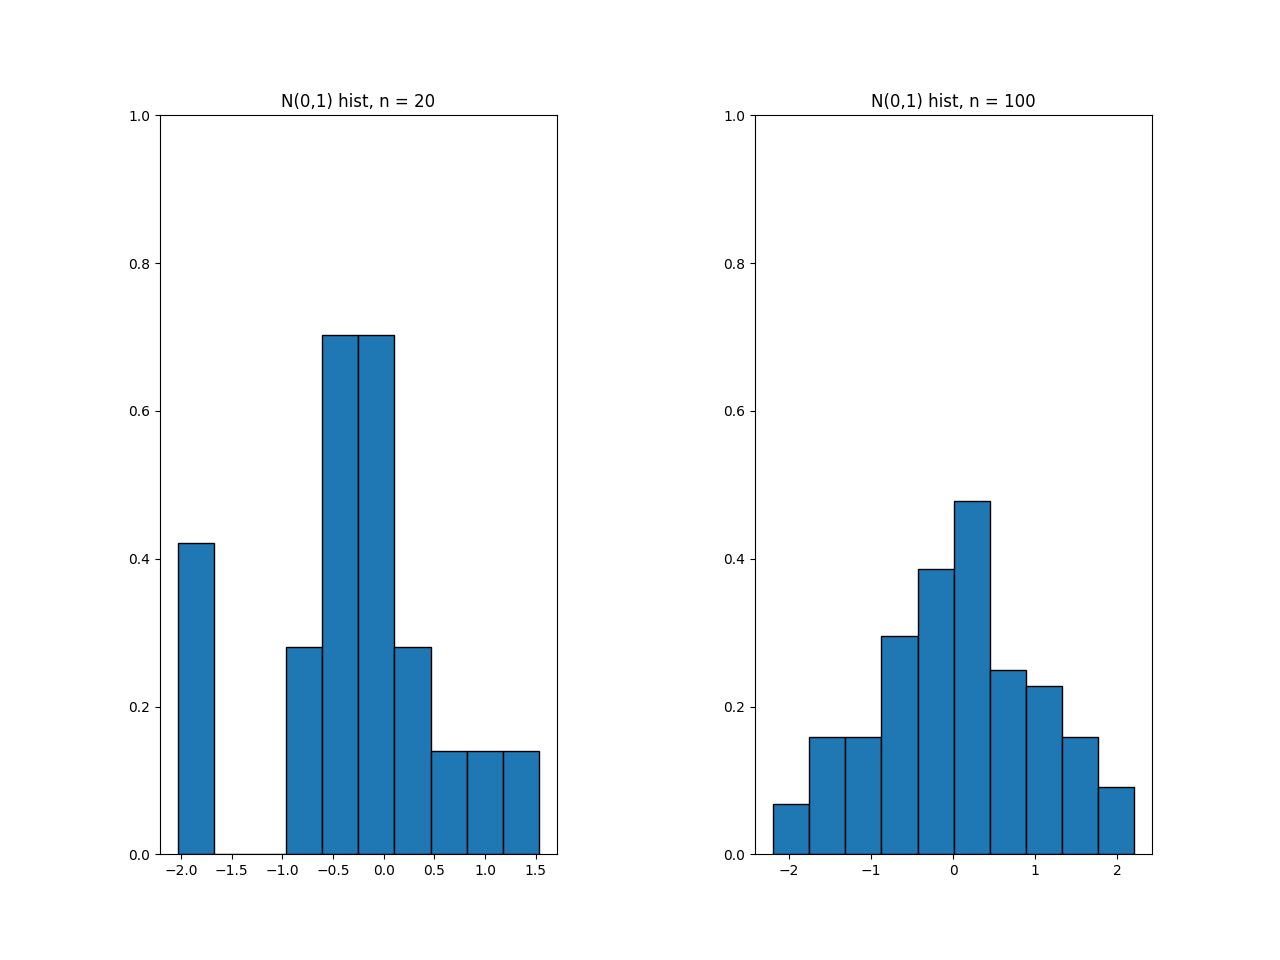
\includegraphics[width=1\linewidth]{task4\_data/hist}}
	\caption{Гистограмма распределения}
	\label{fig:hist}
\end{figure}
\begin{figure}[H]
	\center{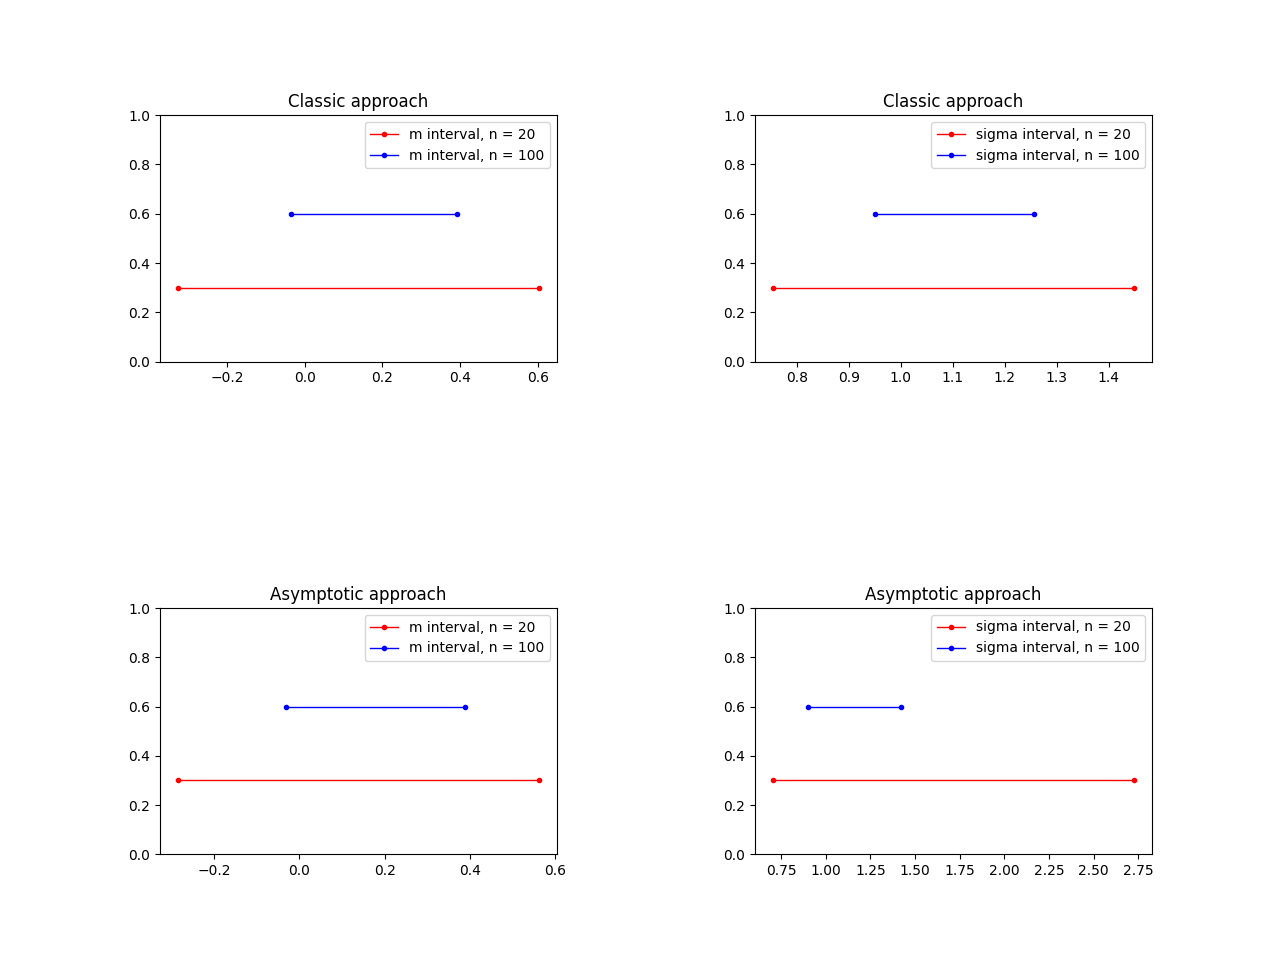
\includegraphics[width=1\linewidth]{task4\_data/intervals}}
	\caption{Полученные интервалы}
	\label{fig:intervals}
\end{figure}